\chapter{File System Calls}
\label{chp:file_system_calls}
\index{File System Calls}

\section{Scratchpad}
\index{Scratchpad}
There is a specific page of the memory which is reserved to store temporary data. This page is known as the \textit{Scratchpad}. The scratchpad is required since any block of the disk cannot be accessed directly  by a process. It has to be present in the memory for access. Hence, any disk block that has to be read or written into is first brought into the scratchpad. It is then read or modified and written back into the disk (if required).

The page 1 of the memory (fig~\ref{fig:main memory}) is used as the scratchpad. Once the OS has booted up there is no need for the OS startup code. So this page can be reused as the scratchpad.

\section{Global File Table and Local File Table}
Before explaining the system calls, we introduce two data structures : \textit{Global File Table} and \textit{Local File Table}.
\begin{itemize}
	\item \textbf{Global File Table} \label{lbl:gft} \index{Process Data Structures!Global File Table}
	 It is a table consisting of a list of all the open files in the system. Refer fig~\ref{fig:main memory} for location in memory. Since each of the 12 processes can open 4 files at a time, this table consists of a maximum of 48 entries. Each entry of the global file table has the following structure as shown in figure~\ref{fig:gft}.

	 \begin{figure}[h!]
		 \centering
			\begin{tabular}{|c|c|}
				\hline
				FAT Index Entry & lseek\\
				\hline
			\end{tabular}
		 \caption{Structure of a GFT entry}
		 \label{fig:gft}
	 \end{figure}

	 \begin{itemize}
		 \item \textbf{FAT index entry :} \index{File Allocation Table!Memory copy} It is used to index the memory copy of the file allocation table(section~\ref{sec:fat}) to get information about that particular file.
		 \item \textbf{lseek :} It is used to get the current position of the next character that will be read from the file. By default, when a file is opened, this parameter has a value 0.
	 \end{itemize}

	\item \textbf{Local File table} \label{lbl:lft} \index{Process Data Structures!Local File Table}
	In addition to the fields discussed earlier(section~\ref{sec:pcb}), the PCB has an additional field known as the \emph{Local File Table}. The local file table consists of 4 entries each of size one word. Each entry corresponds to a file opened by that particular process and stores the global file table index of that file. Thus a process can open a maximum of 4 files. 
	
	The local file table is indexed by a \textit{file descriptor}(an integer value ranging from 0 to 3).
\end{itemize}

\section{Modifications in the OS Startup Code}
\begin{itemize}
	\item The Global File Table in the memory must be initialised with NULL values.

	\item The Local File Table entries in the PCB of the INIT process must be initialised with NULL values.
\end{itemize}

\section{File System Calls}
\label{fssyscall}
\textit{File system calls} are used by a process when it has to create, delete or manipulate \textit{Data files} that reside on the disk(file system). There are seven file system calls. An interrupt is associated with each system call. All the necessary arguments for a system call are available in the user stack with the system call number as the last argument.\\

\noindent Interrupt specifications for different \textit{File system calls} are as follows:

\subsection{INT 1}
The file system calls \textit{Create}, \textit{Open}, \textit{Close} and \textit{Delete} invoke INT 1. INT 1 handles these system calls as follows.
\begin{enumerate}
	\item  \textbf{Create :} This system call is used to create a new file in the file system whose name is specified in the argument.\\
	Syntax : \texttt{int Create(fileName)} \\
	Syscall no : \counter{syscall}
	\index{File System Calls!Create}
	\begin{itemize}
		\item First of all, the memory copy of the FAT \index{File Allocation Table!Memory copy} is searched for a free entry. If no free entry is found, an appropriate error code is returned.
		
		\item Next, the memory copy of the disk free list \index{Disk Free List!Memory copy} is searched to find a free block number.If no free block is found, an appropriate error code is returned. This block is used as the basic block of the file to be created.
		
		\item The \texttt{fileName} specified in the argument and the free block number obtained in the previous step are stored in the \emph{file name} field and \emph{basic block number} field of the free FAT entry, respectively.
				
		\item The \emph{file size} field of the FAT entry is initialized to zero.
		
		\item Each entry of the block list in the basic block is initialized to zero.\footnote{This can be achieved by loading the basic block into the scratchpad, updating it and then committing back the updated basic block.}
		
		\item The updated copies of FAT \index{File Allocation Table!Memory copy} and disk free list 
		\index{Disk Free List!Memory copy} in the memory are committed to the disk.
		
		\item The return value of this system call is 0 in case of success and the appropriate error code in case of failure.
	\end{itemize}

	\item \textbf{Open :} This system call is used to open an existing file whose name is specified in the argument.\\
	Syntax : \texttt{int Open(fileName)} \\
	Syscall no : \counter{syscall} 
	\index{File System Calls!Open}
	\begin{itemize}
		\item  First of all, a free entry is searched in the local file table of the process. If there are no free entries, in the case where a process already has 4 open files, an appropriate error code is returned.
		
		\item Then, the global file table is searched for a free entry. If there is no free entry, an appropriate error code is returned else a new global file table entry is created and the fields are filled with appropriate values in the following manner:
		\begin{itemize}
			\item The memory copy of FAT \index{File Allocation Table!Memory copy} is searched using the \texttt{fileName} and the corresponding index of that file in the FAT \footnote{By index, we mean the sequential position (starting from 0) of that entry in the data structure mentioned.} is stored as the \emph{FAT index}. If the file does not have an entry in the FAT, an appropriate error code is returned.
			
			\item The \emph{lseek} field is set to zero.
		\end{itemize}
		
		\item The index of this global file table entry is stored in its local file table.
		
		\item The index of this entry in the local file table is returned as a return value of the system call. This is known as the file descriptor.
	\end{itemize}

	\item  \textbf{Close :} This system call is used to close an open file. The file can only be closed by the process which opened it or by its children. \\
	Syntax : \texttt{int Close(fileDescriptor) } \\
	Syscall no : \counter{syscall}
	\index{File System Calls!Close}
	\begin{itemize}
		\item The \texttt{fileDescriptor} is used first to access the local file table entry of the file. An appropriate error code is returned if the \texttt{fileDescriptor} is out of the range specified.
		
		\item The global file table entry indexed by this local file table entry is removed. \footnote{A suggested way to remove an entry is to store an integer -1 in that word.} %TODO -1 or ''\0``
		
		\item The local file table entry of the process is then removed.
		
		\item The return value of this system call is 0 in case of success and the appropriate error code in case of failure.
	\end{itemize}

	\item \textbf{Delete :} This system call is used to delete the file from the file system whose name is specified in the argument. \\
	Syntax : \texttt{int Delete(fileName)} \\
	Syscall no : \counter{syscall}
	\index{File System Calls!Delete}
	\begin{itemize}
		\item The memory copy of the FAT \index{File Allocation Table!Memory copy} is searched using the \texttt{fileName} to get the corresponding FAT entry. If no entry is found, an appropriate error code is returned.
		
		\item If the file is already open an appropriate error code is returned. We adopt the following steps to check if the file is open.
		\begin{itemize}
			\item The \emph{FAT index entry} of each global file table entry is used to fetch the filename of the corresponding open file from the memory copy of the FAT \index{File Allocation Table!Memory copy}.
			
			\item Each of the filenames obtained in the previous step is compared with the \texttt{fileName}. If match is found, we conclude that the file is currently in open.
		\end{itemize}
		\item The \emph{basic block number} field in this FAT entry obtained, is then used to load the basic block of the file into the scratchpad.
		
		\item Each entry in the block list of the basic block is used to find the data blocks of the file. Then, entries in the memory copy of the disk free list \index{Disk Free List!Memory copy}  corresponding to these data blocks are set to zero, thereby freeing them.
		
		\item Finally, the FAT entry of the file is removed.
		
		\item The updated copies of FAT \index{File Allocation Table!Memory copy} and disk free list \index{Disk Free List!Memory copy} in the memory are committed to the disk.
		
		\item The return value of this system call is 0 in case of success and the appropriate error code in case of failure.
	\end{itemize}
\end{enumerate}

\subsection{INT 2}
The file system calls \textit{Read}, \textit{Write} and \textit{Seek} invoke INT 2. INT 2 handles these system calls as follows.
\begin{enumerate}
	\item \textbf{Write :} This system call is used to write data into an open file. \\
	Syntax : \texttt{int Write(fileDescriptor, mem\_loc, numWords)} 
	\footnote{It is advisable to have  a maximum of 1 block 
	for any data file if it has to be modified using \texttt{write} system call since if the modification spans 
	multiple blocks the entire procedure to access a block (outlined above) has to be repeated.} \\ 
	Syscall no : \counter{syscall}
	\index{File System Calls!Write}
	\begin{itemize}
		\item First of all, the basic block of the file specified by the \texttt{fileDescriptor} is loaded into the scratchpad. This is done in the following way:
		\begin{itemize}
			\item The \texttt{fileDescriptor} is used first to access the local file table entry of the file. An appropriate error is returned if the \texttt{fileDescriptor} is out of the range specified.
			\item This local file table entry is then used to access the global file table entry of the file.
			\item Then the FAT index field in the global file table entry is used to access the FAT entry of the file.
			\item The basic block address present in the FAT entry is then used load the basic block (containing block list and file header info) into the scratchpad. Refer figure~\ref{access_scheme}.
		\end{itemize}	
		\item The lseek position present in the GFT entry and \texttt{numWords} are used to index the block list in the basic block to find the block numbers of the block(s) to be written into. \footnote{The data block to which the lseek position is pointing to is got by dividing lseek by the block size. \\
		The data block number calculated above is used to index the block list in the basic block to get the exact location of the data block in the disk. The data block is then loaded from the disk into the scratchpad. \\
		If the words to be read are split across multiple data blocks, the above procedure is repeated.}
		\item Each time the block to be written into is loaded into the scratchpad before performing the write operation.
		\item After loading the specified block, the content to be written is copied from the user memory location (\texttt{mem\_loc}) into this block. If \texttt{mem\_loc} is out of the address space of the process, an appropriate error code is returned.
		\item If the write operation exhausts all the currently allocated blocks, new blocks are allocated as required. This is done in the following way.
		\begin{itemize}
			\item The memory copy of the disk free list \index{Disk Free List!Memory copy} is used to get the block number of a free block.
			\item A new basic block entry is created using this free block number and added to the block list of the basic block. Successive write operations are then performed the usual way.
		 \end{itemize}
		\item Once all the write operations are over for that block, it is stored back into the disk.
		\item The updated copies of FAT \index{File Allocation Table!Memory copy} and disk free list \index{Disk Free List!Memory copy} in the memory are committed to the disk.
		\item The return value of this system call is the number of words successfully written. In case of an error, an appropriate error code is returned.
		\end{itemize}
	
	\item \textbf{Seek :} This system call is used to change the current value of the seek position in the global file table entry of a file. \\
	Syntax : \texttt{int Seek(fileDescriptor, lseek)}  \\
	Syscall no : \counter{syscall}
	\index{File System Calls!Seek}
	\begin{itemize}
		\item The \texttt{fileDescriptor} is used first to access the local file table entry of the file. An appropriate error code is returned if the \texttt{fileDescriptor} is out of the range specified.
		\item This local file table entry is then used to access the global file table entry of the file.
		\item Then the FAT index field in the global file table entry is used to access the FAT entry of the file.
		\item The \emph{file size} got from this FAT entry is checked to be greater than \texttt{lseek}. Otherwise an appropriate error code is returned.\footnote{Seek is allowed only \emph{within} a file.}
		\item The \emph{lseek} field in the GFT entry is then changed to the new value specified in the argument (\texttt{lseek}).
		\item The return value of this system call is 0 in case of success and the appropriate error code in case of failure.
	\end{itemize}
	
	\item \textbf{Read :} This system call is used to read data from an open file.\\
	Syntax : \texttt{int Read(fileDescriptor, mem\_loc, numWords)} \\
	Syscall no : \counter{syscall}
	\index{File System Calls!Read}
	\begin{itemize}
		\item First of all, the basic block of the file specified by the \texttt{fileDescriptor} is loaded in the scratchpad. This is done in the following way:
		\begin{itemize}
			\item The \texttt{fileDescriptor} is used first to access the local file table entry of the file. An appropriate error is returned if the \texttt{fileDescriptor} is out of the range specified.
			\item This local file table entry is then used to access the global file table entry of the file. 
			\item Then the \emph{FAT index} field in the global file table entry is used to access the FAT entry of the file.
			\item The basic block address present in the FAT entry is then used to load the basic block (containing block list and file header info) into the scratchpad. Refer figure~\ref{access_scheme}.
		\end{itemize}	
		\item The \emph{lseek} position present in the GFT entry and \texttt{numWords} are used to index the block list in the basic block to find the address of the block(s) to be read.
		\item Each time the block to be read is loaded into the scratchpad before reading its contents.
		\item The contents read are then copied into the buffer that is specified as an argument to the system call (\texttt{mem\_loc}). If the \texttt{mem\_loc} is out of the address space of the process, an appropriate error code is returned.
		\item The return value of this system call is the number of words successfully read. In case of an error, an appropriate error code is returned.
	\end{itemize}

	\begin{figure}[htp!]
		\centering
		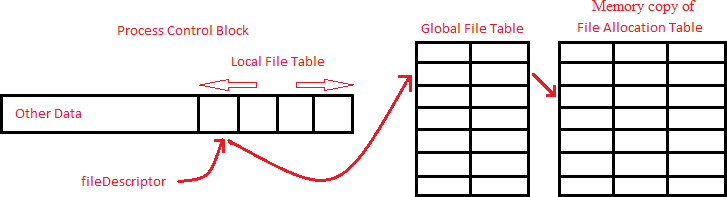
\includegraphics[scale=0.65]{pics/access_method}
		\caption{Diagram showing the method of accessing FAT entry}
		\label{access_scheme}
	\end{figure}
\end{enumerate}
